This section presents the effect of pileup events on the isolation of the leptons 
produced in the primary interaction. The presence of additional inelastic
interactions is expected to add some additional energy to the isolation cone
of the leptons from the primary interaction, thus decreasing the efficiency
of the isolation cut on signal events. This decrease in efficiency can be 
studied as a function of the number of reconstructed primary vertices, serving
as a reasonable measure of the number of additional pileup interaction.

A number of techniques exist to correct for this inefficiency due to pileup,
which are still under investigation at the moment. For the current analysis, 
we do not perform any pileup correction for isolation and quantify the loss
in this section.

\begin{figure}[!htbp]
\begin{center}
\subfigure[Barrel ]{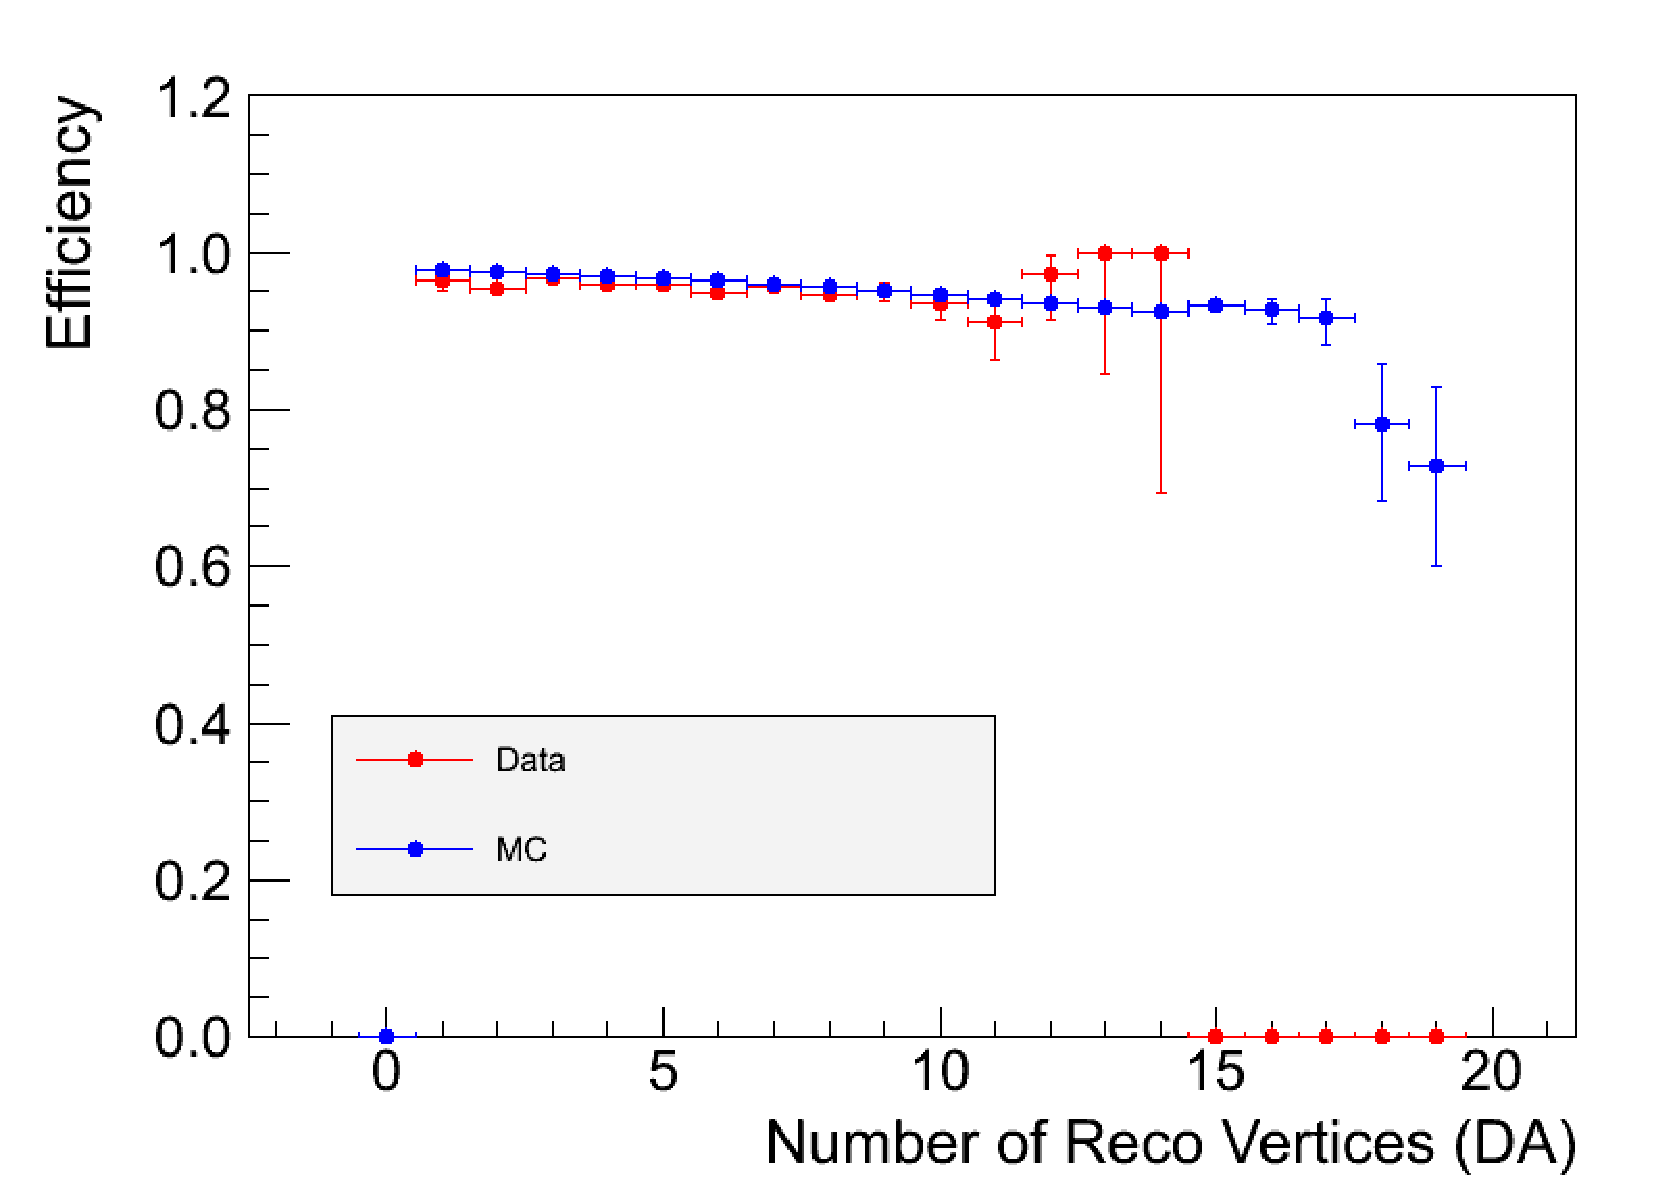
\includegraphics[width=0.45\textwidth]{figures/ElectronIsolationBarrelEffVsNVertices_TagAndProbe.pdf}}
\subfigure[Endcap]{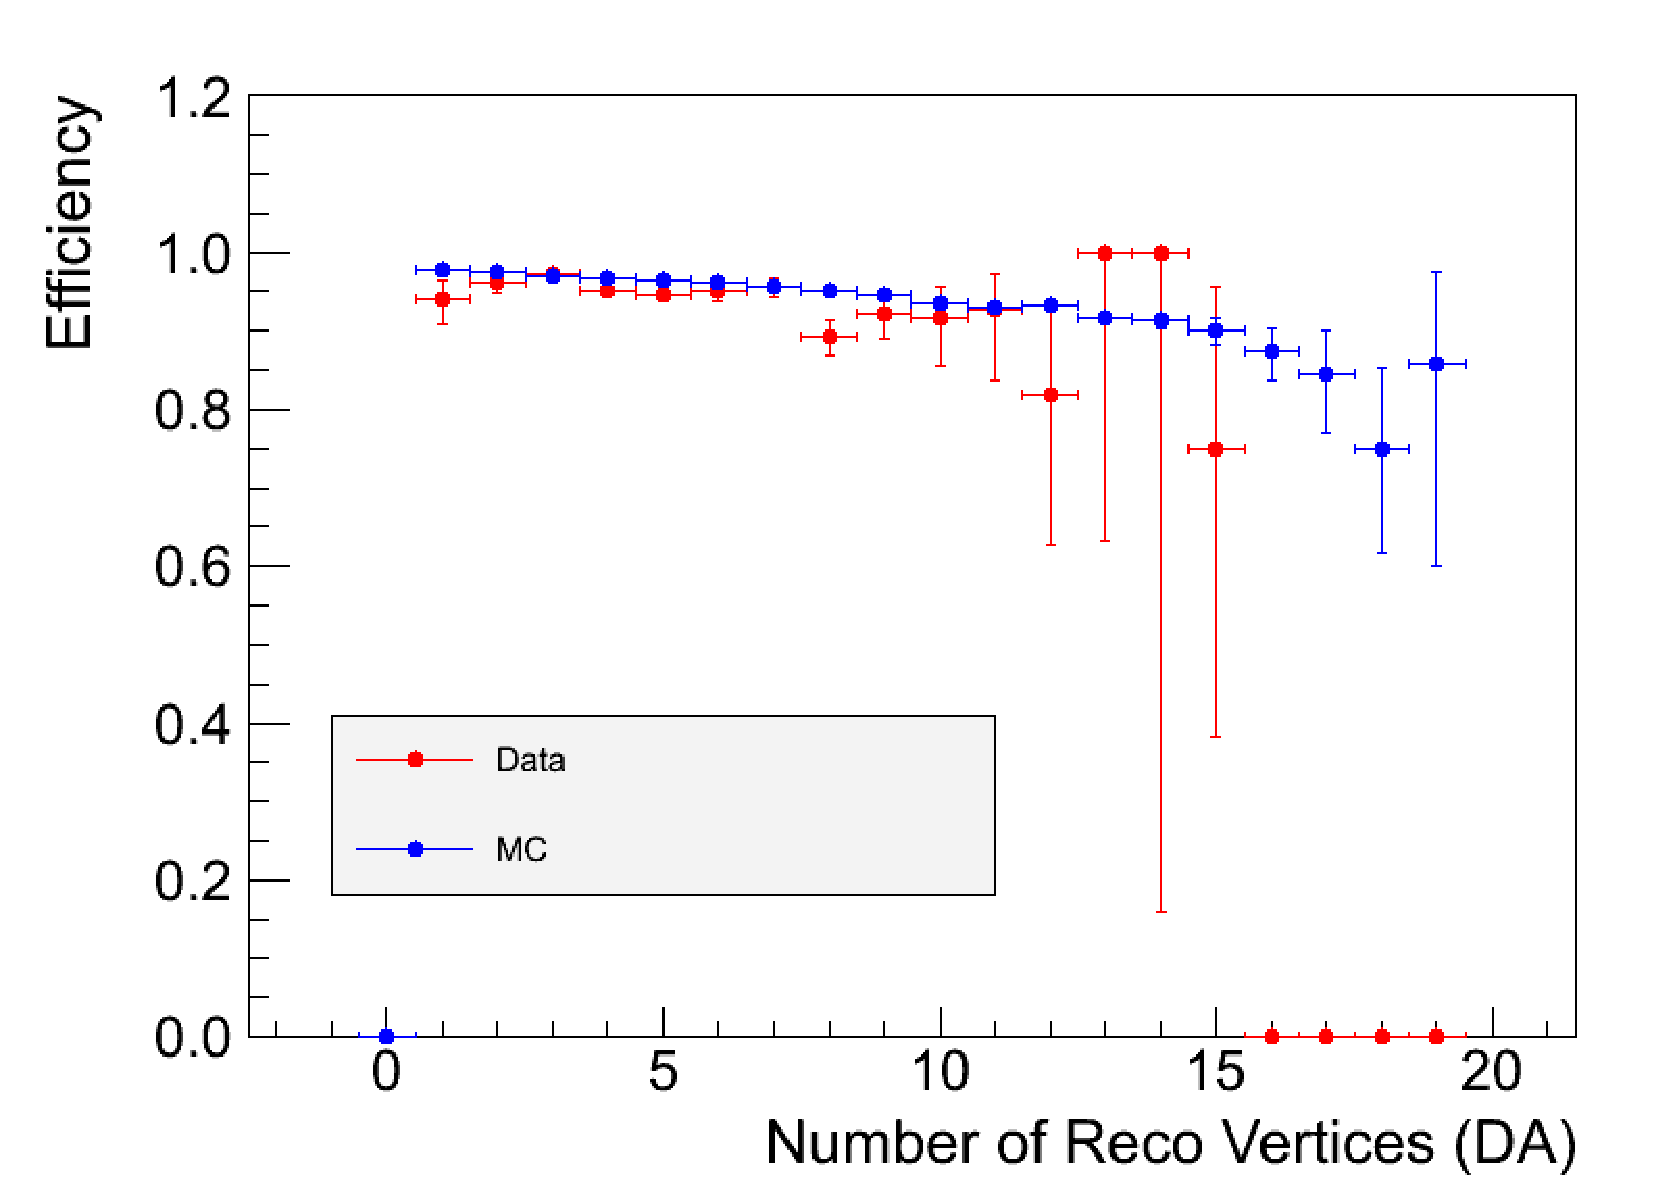
\includegraphics[width=0.45\textwidth]{figures/ElectronIsolationEndcapEffVsNVertices_TagAndProbe.pdf}}
\caption{Isolation efficiency vs number of reconstructed primary vertices for electrons, comparing the 
results from the tag and probe selection on 2011 data with the Z Monte Carlo simulation.}
\label{fig:eleIsoEff_TagAndProbe_vs_NVertices}
\end{center}
\end{figure}

\begin{figure}[!htbp]
\begin{center}
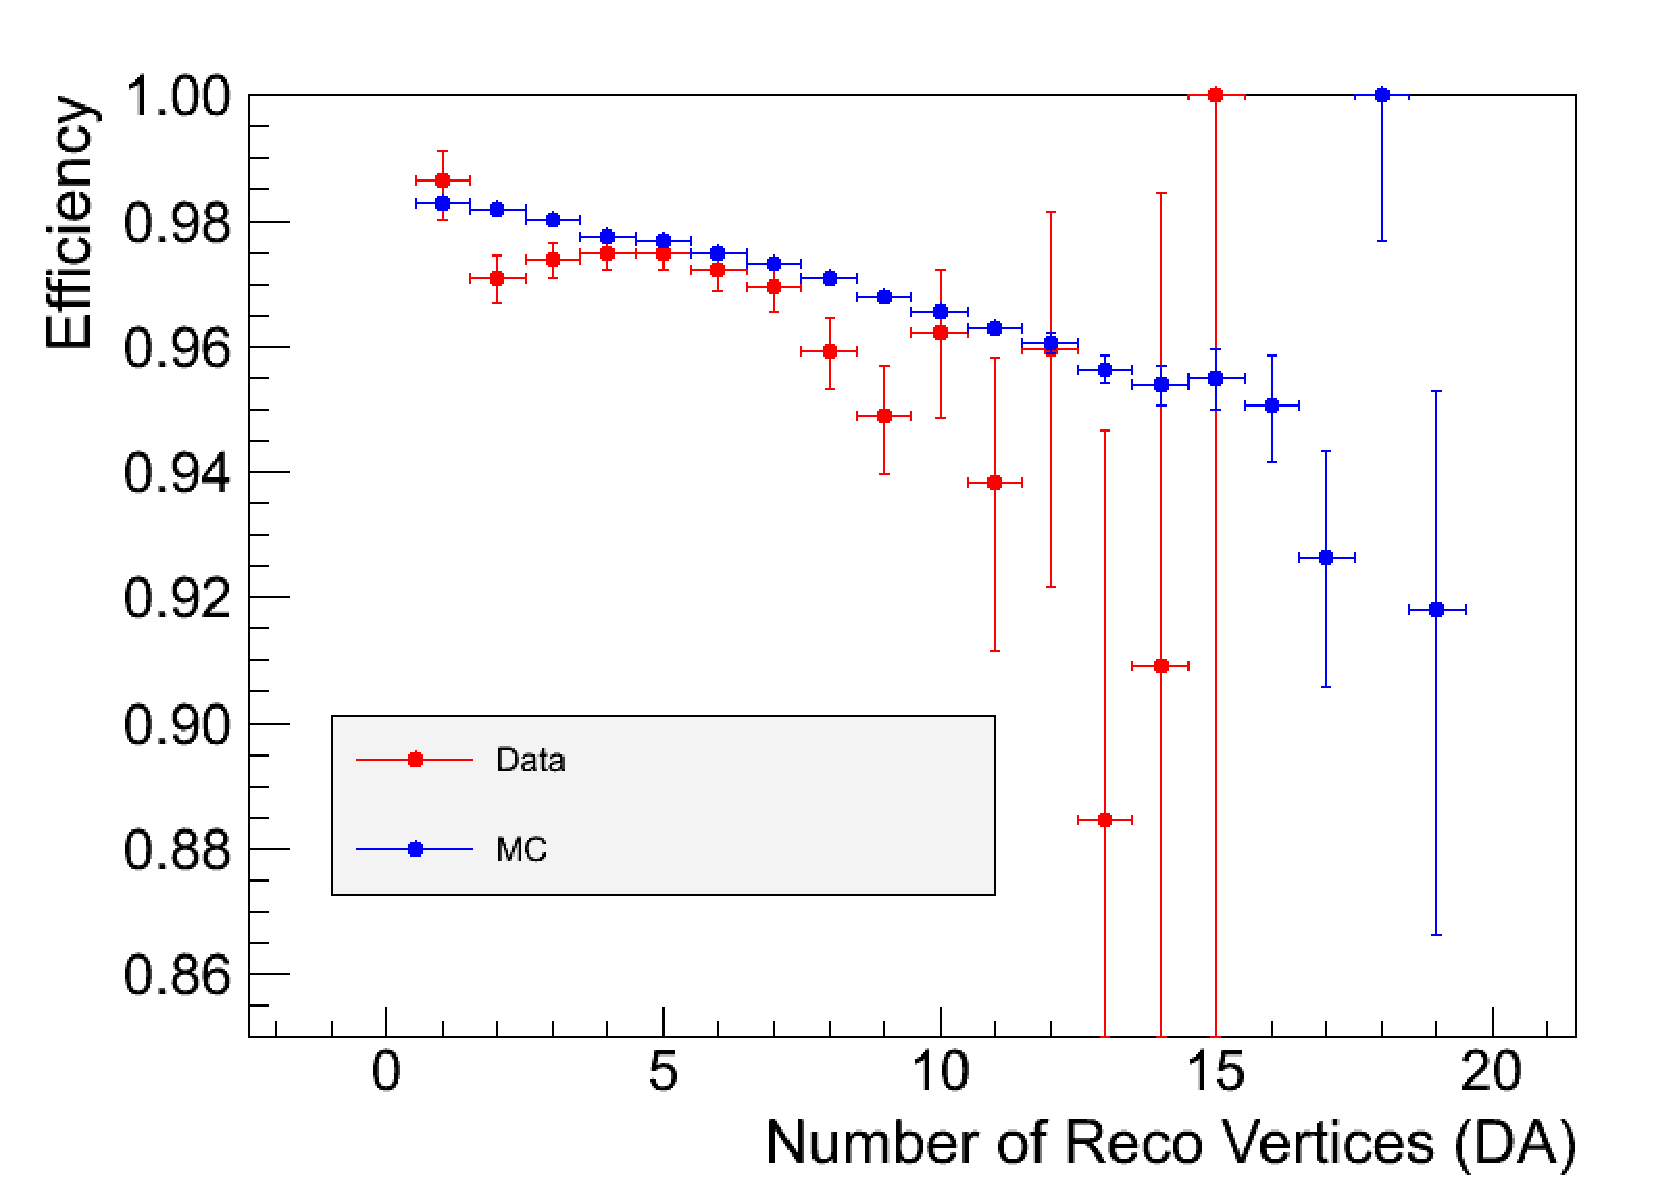
\includegraphics[width=0.45\textwidth]{figures/MuonIsolationEffVsNVertices_TagAndProbe.pdf}
\caption{Isolation efficiency vs number of reconstructed primary vertices for muons, comparing the 
results from the tag and probe selection on 2011 data with the Z Monte Carlo simulation.}
\label{fig:muIsoEff_TagAndProbe_vs_NVertices}
\end{center}
\end{figure}

Figs. \ref{fig:eleIsoEff_TagAndProbe_vs_NVertices} and \ref{fig:muIsoEff_TagAndProbe_vs_NVertices} 
show the isolation efficiency for electrons and muons respectively, measured using the
tag and probe selection, for 2011 data and Z Monte Carlo simulation. Agreement in these
efficiencies allow us to use the signal Monte Carlo to infer the efficiency loss under 
high pileup environment. The lepton isolation efficiency for HWW signal events are plotted
in Fig \ref{fig:HWW130IsoEff_vs_NVertices}, showing a loss of efficiency of 5\% for 
electrons and 2\% for muons, between events with one reconstructed primary vertex
and 10 reconstructed primary vertices. The efficiency loss for leptons with $p_{T}$ 
between $10$ and $20$ GeV is much larger compared to the efficiency loss for higher
$p_{T}$ leptons. As a result the efficiency loss on signal events is dependent 
on the mass of the Higgs boson. For a signal with Higgs mass of $130$ GeV, 
the average loss of efficiency for electrons and muons with $p_{T}>20$ GeV is
$2\%$ and $1\%$ respectively. 


\begin{figure}[!htbp]
\begin{center}
\subfigure[HWW130 Electrons]{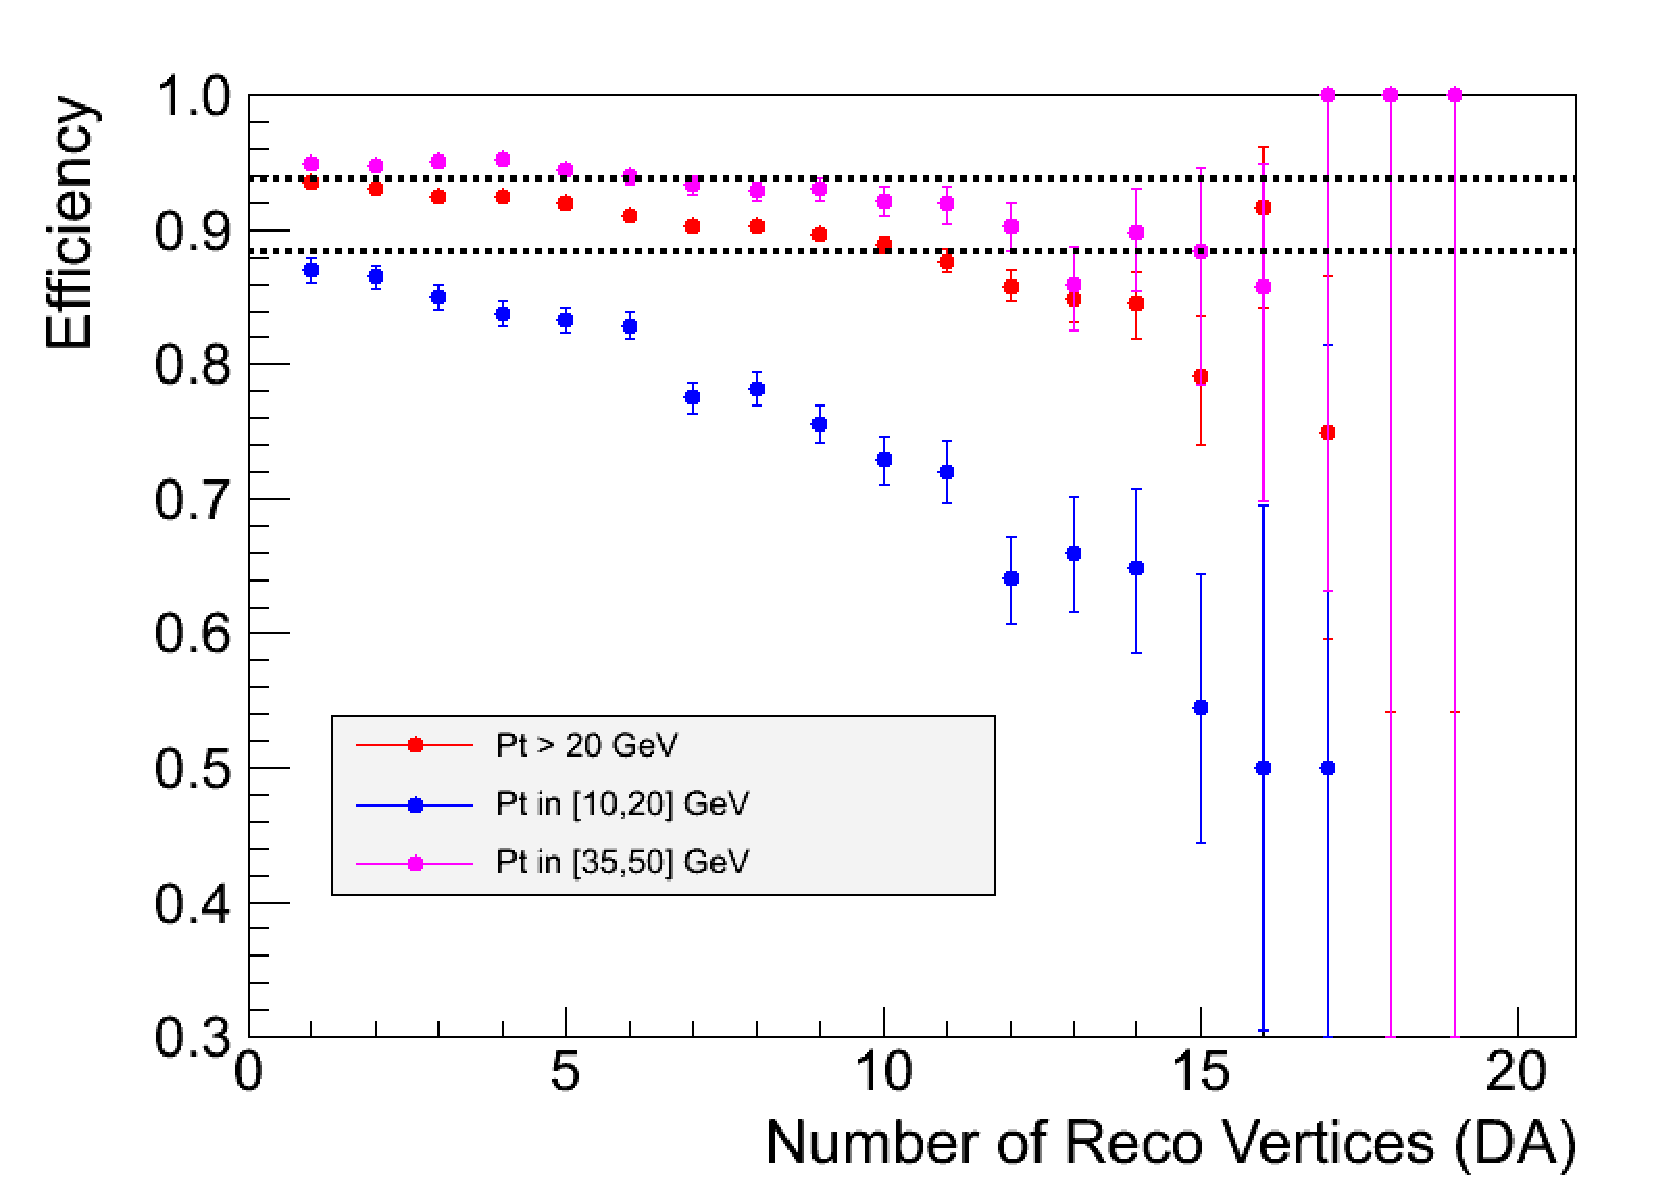
\includegraphics[width=0.45\textwidth]{figures/ElectronIsolationVsNVertices_HWW130.pdf}}
\subfigure[HWW130 Muons]{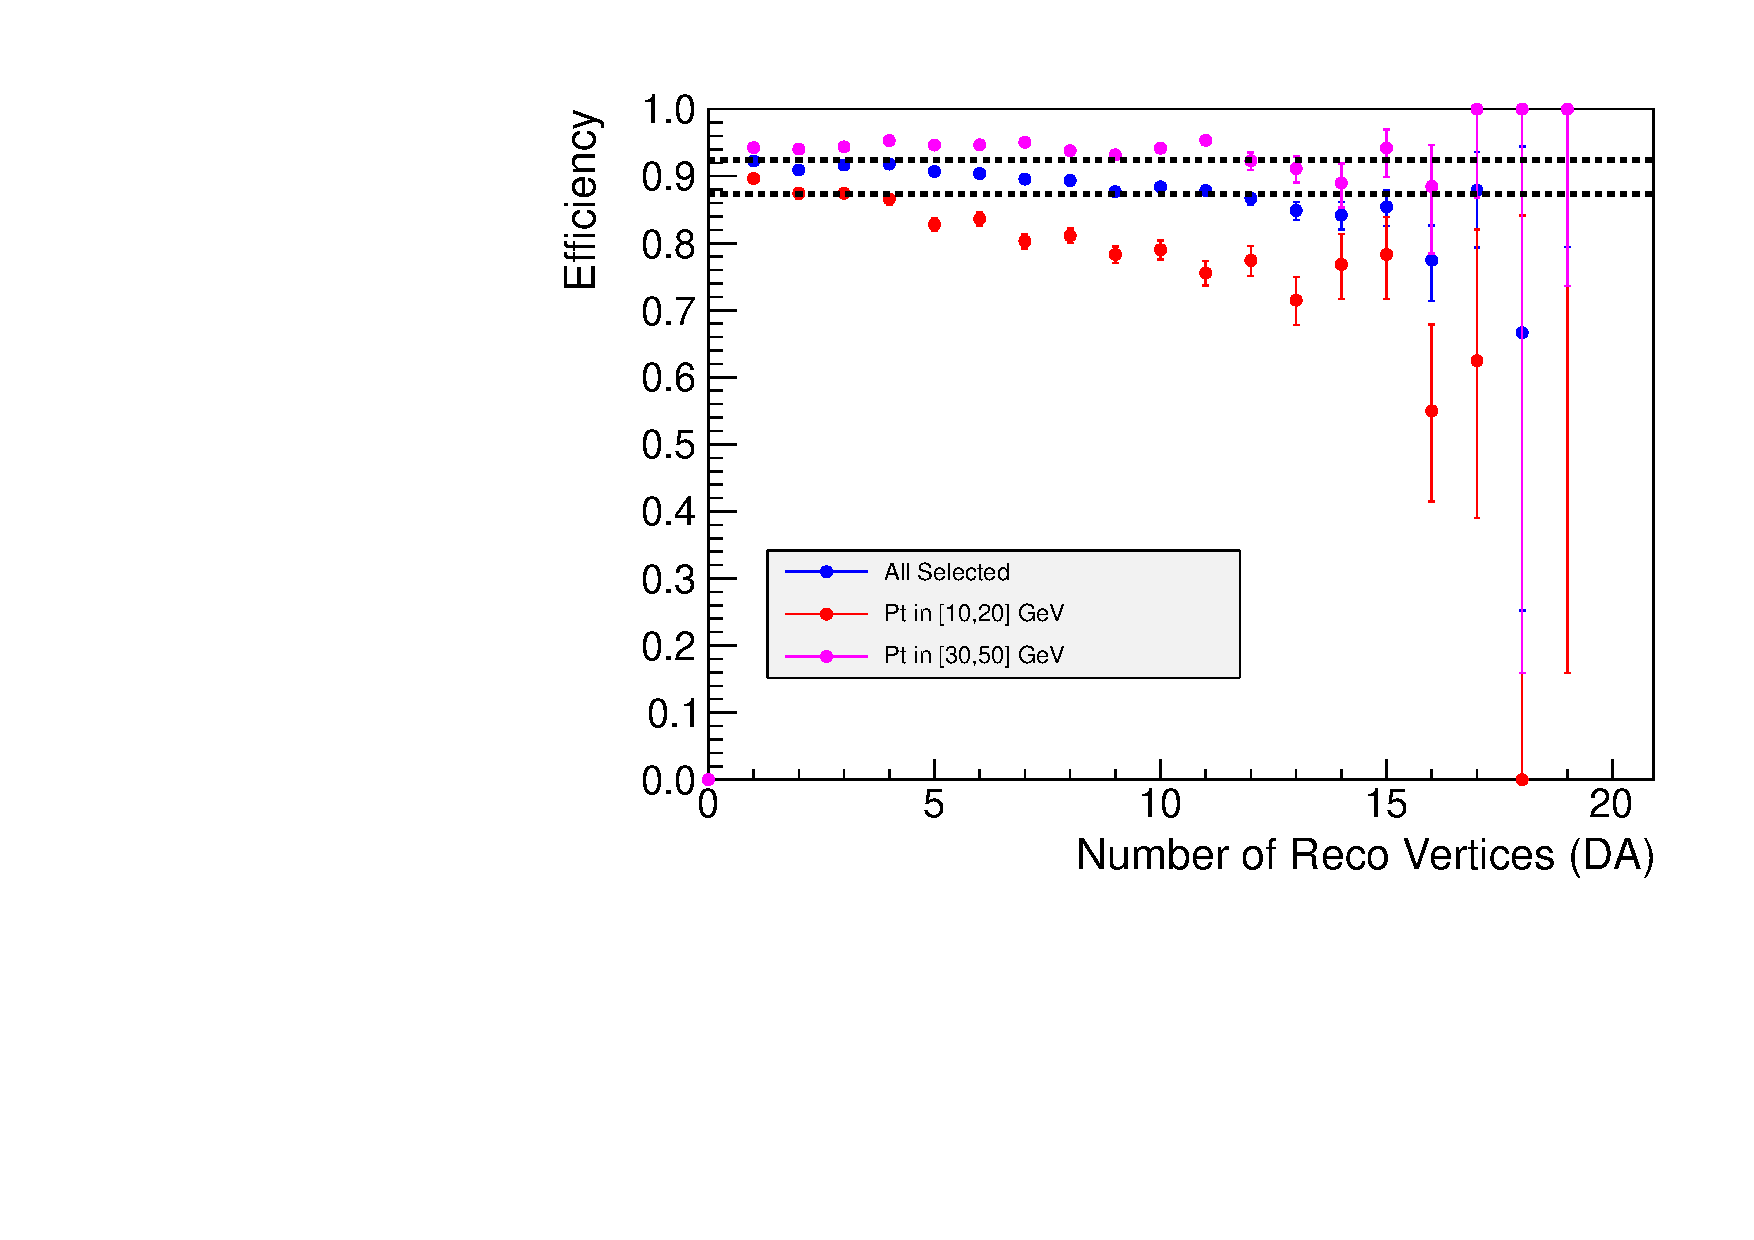
\includegraphics[width=0.45\textwidth]{figures/MuonIsolationVsNVertices_HWW130.pdf}}
\caption{Isolation efficiency vs number of reconstructed primary vertices for electrons and muons
in the HWW ($m_{H} = 130$) Monte Carlo simulation. The isolation efficiency for various $p_{T}$ 
bins are shown.}
\label{fig:HWW130IsoEff_vs_NVertices}
\end{center}
\end{figure}


\begin{figure}[!htbp]
\begin{center}
\subfigure[HWW130 Electrons]{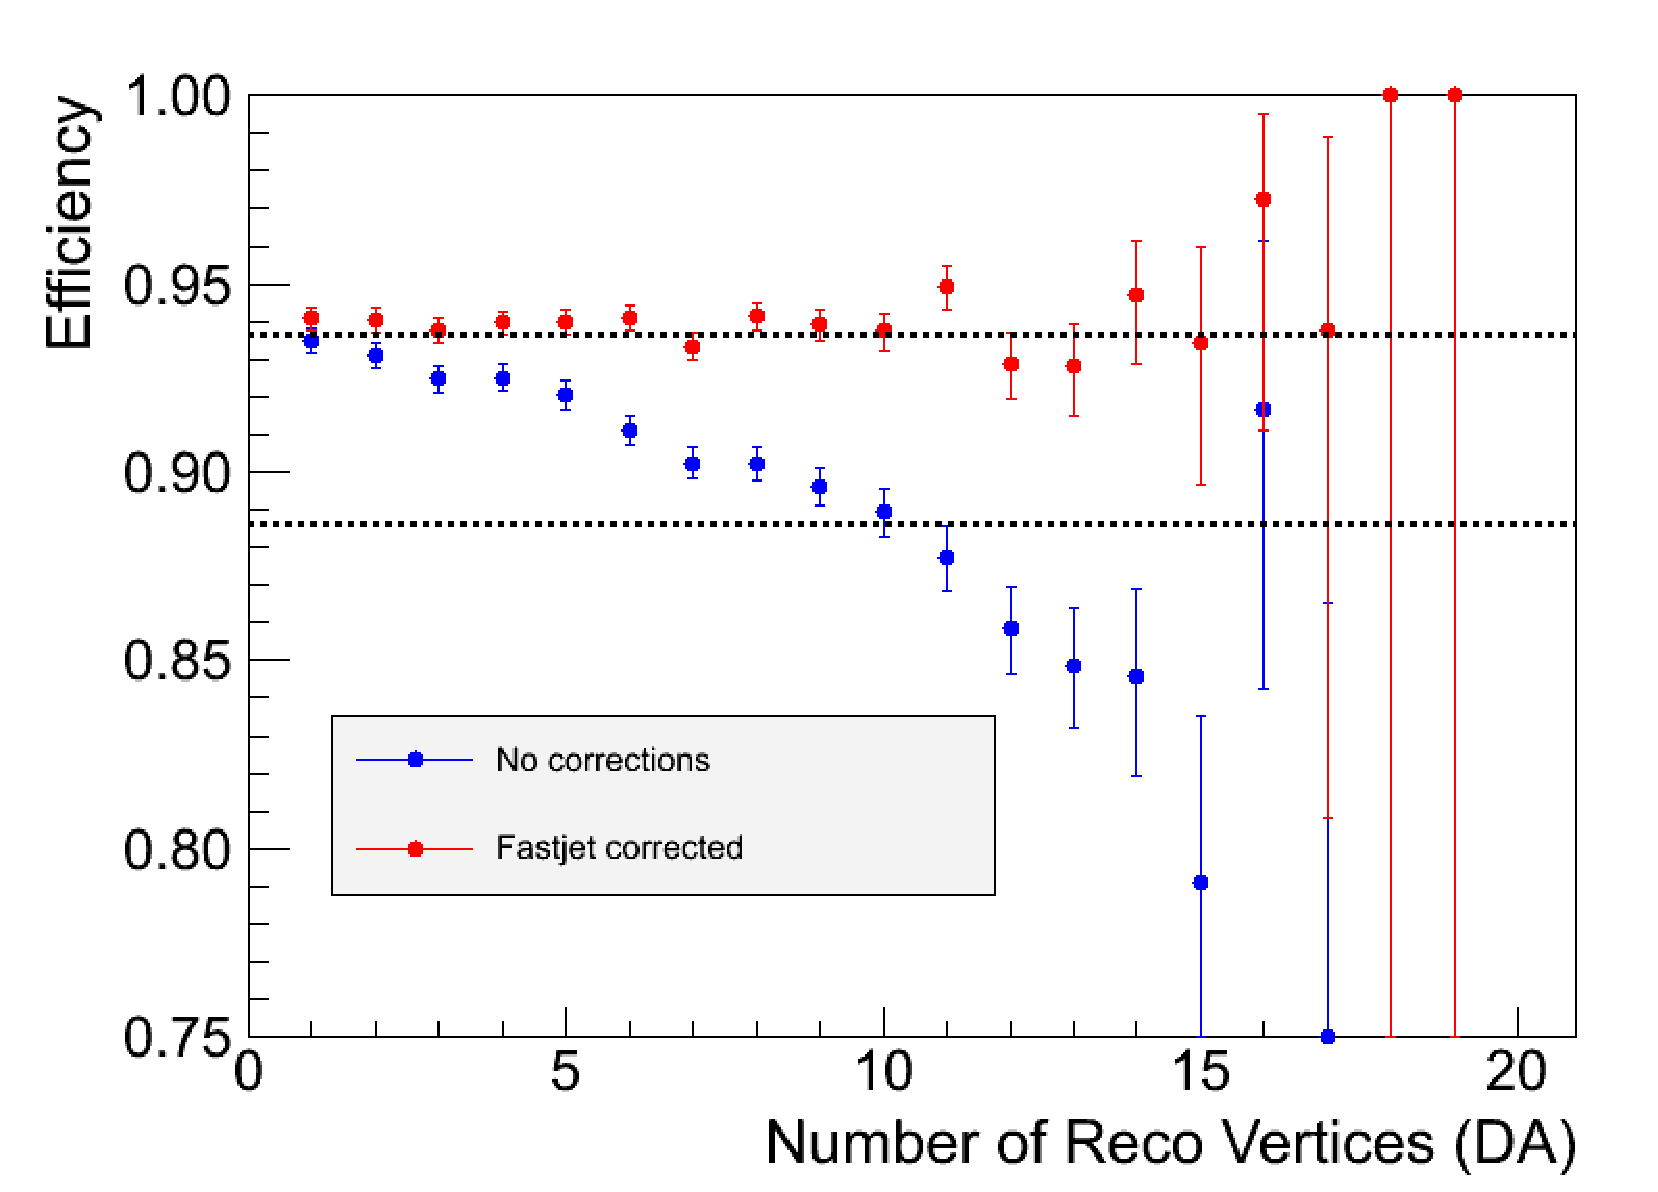
\includegraphics[width=0.45\textwidth]{figures/ElectronIsolationVsNVertices_HWW130_FastjetCorrection.pdf}}
\subfigure[HWW130 Muons]{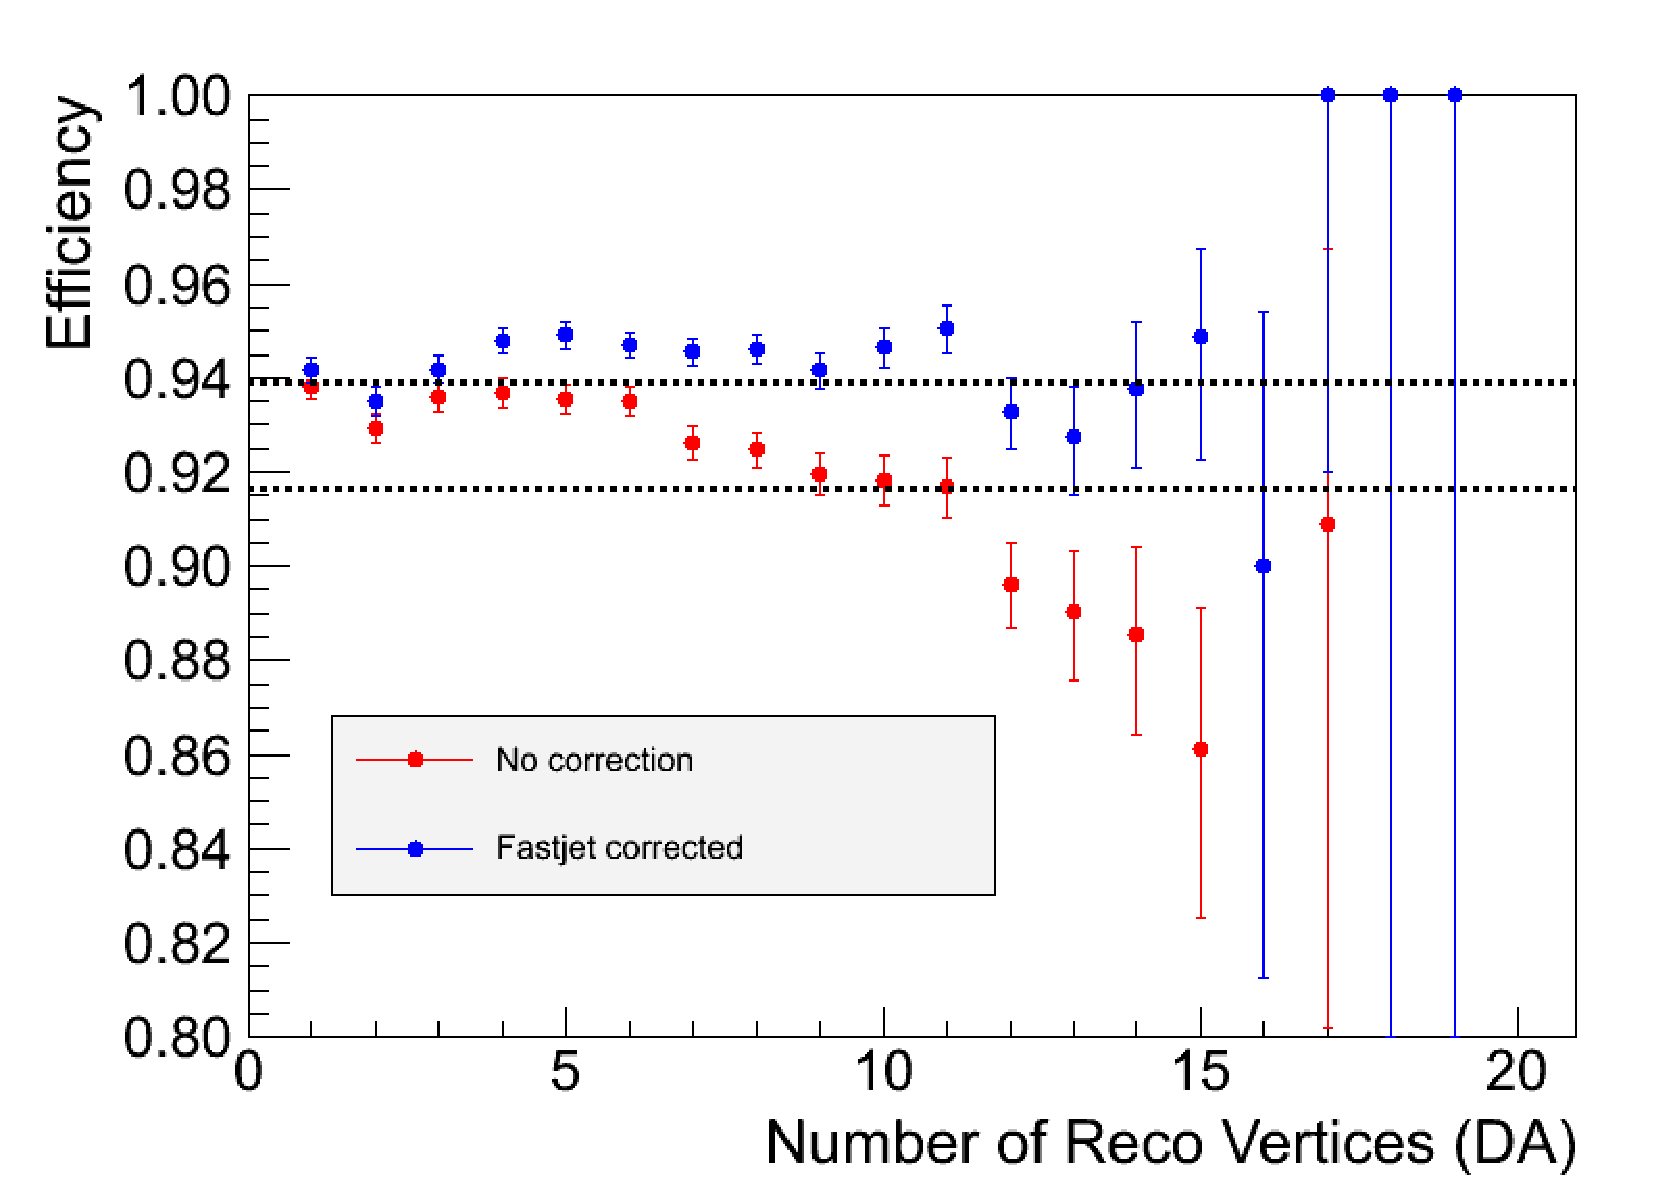
\includegraphics[width=0.45\textwidth]{figures/MuonIsolationVsNVertices_HWW130_FastjetCorrection.pdf}}
\caption{Signal lepton isolation efficiency vs number of reconstructed primary vertices, comparing uncorrected 
and fastjet corrected isolation cuts in the HWW ($m_{H} = 130$) Monte Carlo simulation. Leptons
with $p_{T} > 20$ GeV are used.}
\label{fig:HWW130IsoEff_vs_NVertices_FastjetCorrection}
\end{center}
\end{figure}

\begin{figure}[!htbp]
\begin{center}
\subfigure[Fake rate Data]{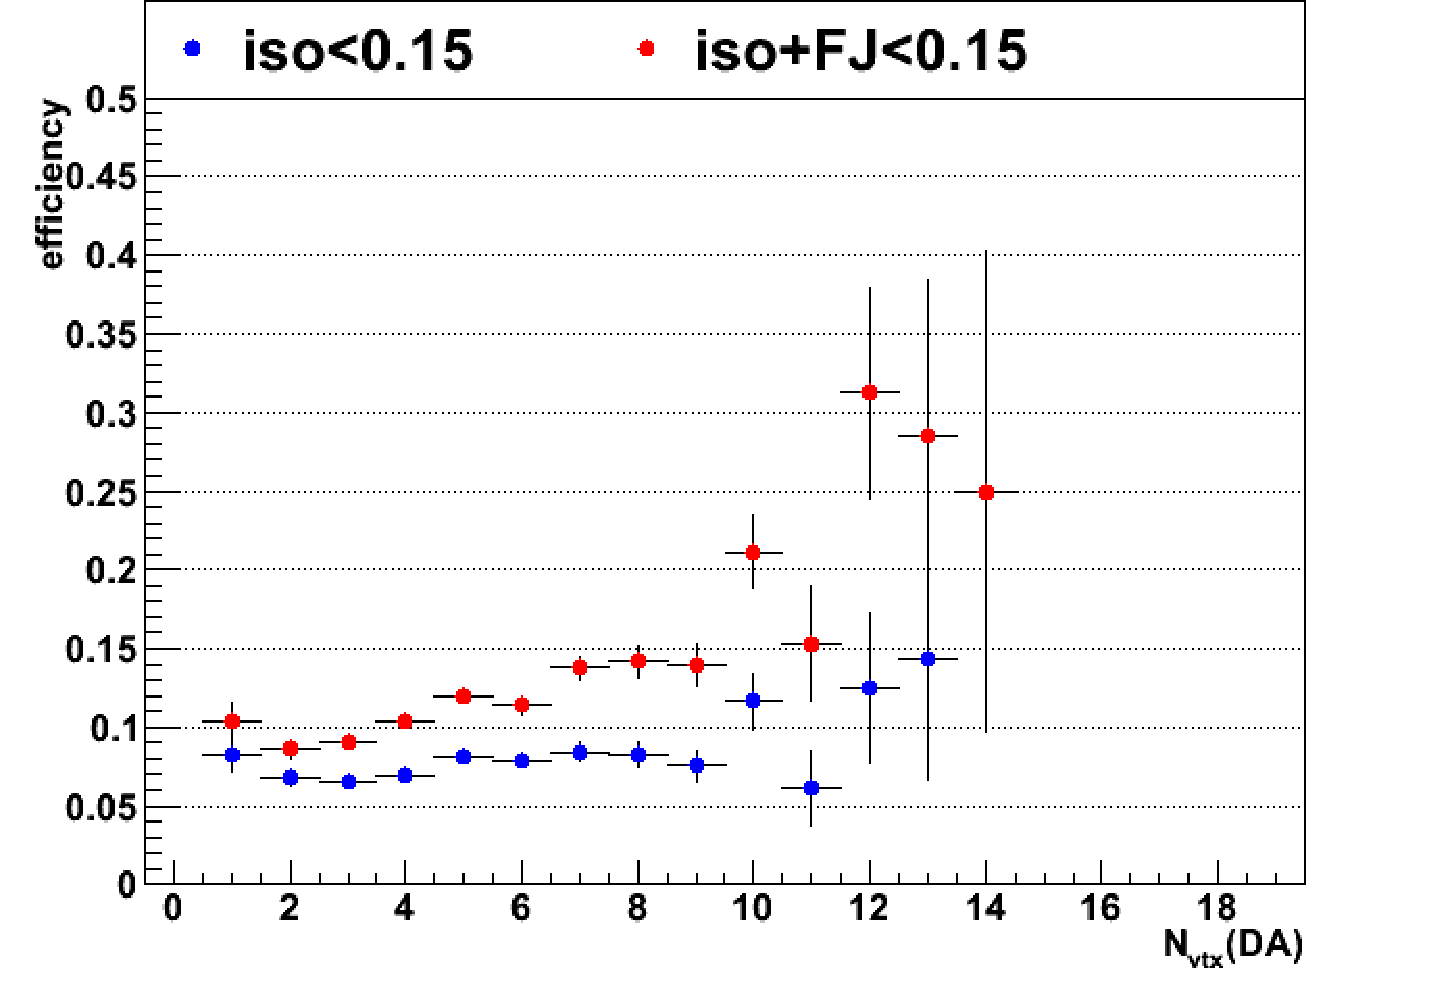
\includegraphics[width=0.45\textwidth]{figures/MuonIsolationVsNVertices_JetData_FastjetCorrection.pdf}}
\subfigure[QCD MC]{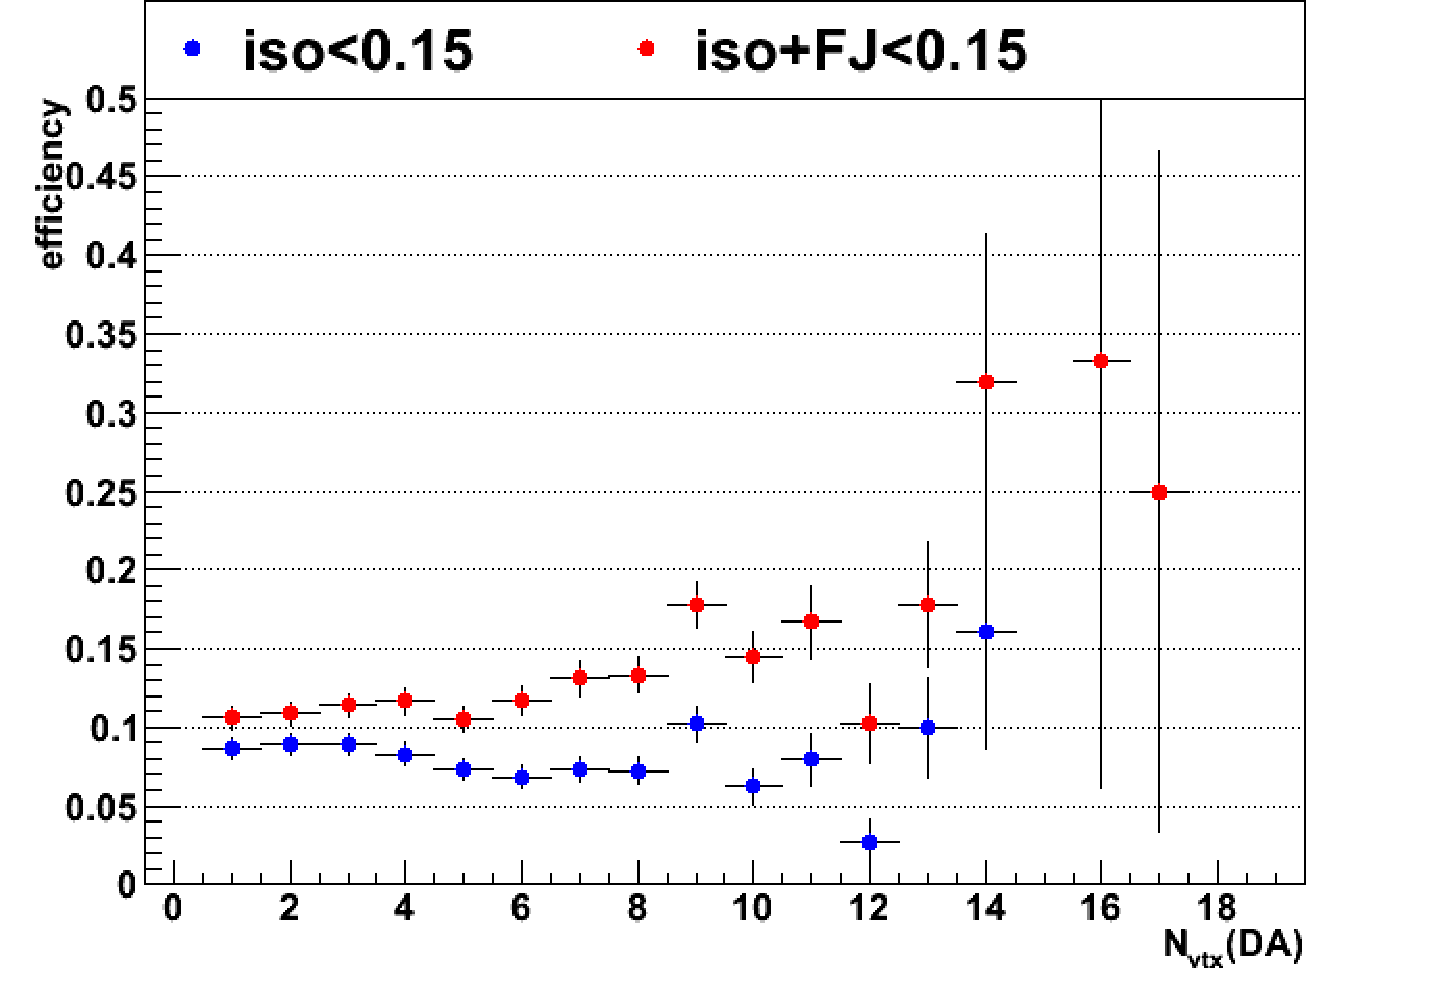
\includegraphics[width=0.45\textwidth]{figures/MuonIsolationVsNVertices_QCDMC_FastjetCorrection.pdf}}
\caption{Background lepton isolation efficiency vs number of reconstructed primary vertices, comparing uncorrected 
and fastjet corrected isolation cuts. Results for a fake lepton dominated data sample, and the QCD Monte Carlo simulation
are shown. }
\label{fig:BkgIsoEff_vs_NVertices_FastjetCorrection}
\end{center}
\end{figure}


The isolation is one aspect of the analysis that will need to be improved in the future, 
either employing appropriate pileup corrections to recover these inefficiencies, or 
parameterizing and re-tuning the cuts as a function of some observable correlated
to pileup. As a preliminary attempt at pileup corrections for isolation, we investigated
the possiblity to use the fastjet correction described in Section \ref{sec:sel_jets} 
assuming a fixed area corresponding to the isolation cone of $\Delta$R $< 0.3$. 
The isolation efficiency for electrons and muons from HWW signal events are shown in 
Figure \ref{fig:HWW130IsoEff_vs_NVertices_FastjetCorrection}, comparing
the fastjet corrected isolation with the uncorrected isolation as a function of the 
number of reconstructed primary vertices. We observe that the efficiency does indeed become 
flat for signal. However, we observe that for the background leptons, this correction appears
over-correct the pileup contribution, demonstrated by the fact that the efficiency increases
as a function of the number of reconstructed primary vertices shown in Fig 
\ref{fig:BkgIsoEff_vs_NVertices_FastjetCorrection}. Therefore, further studies are needed to 
understand the effect and performance of all the different pileup correction options, and
will be presented as an update to the note in subsequent versions.


